\usetikzlibrary{arrows.meta,calc}
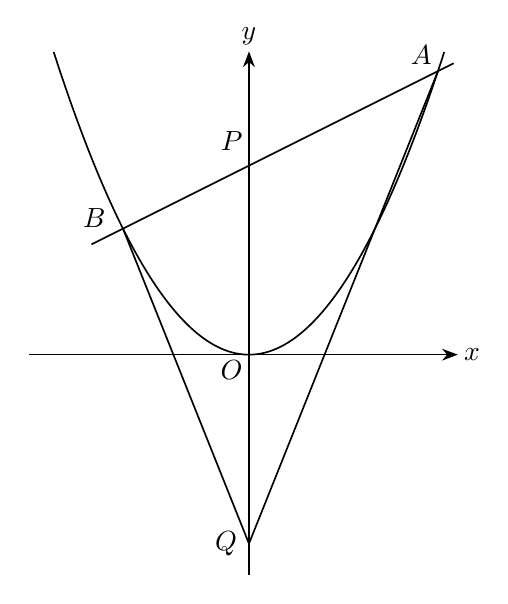
\begin{tikzpicture}[x=1cm,y=1cm,line width=.6pt,font=\normalsize,>=Stealth]
\coordinate (O) at (0,0);
\coordinate (A) at (2.4,3.6);
\coordinate (B) at (-1.6,1.6);
\coordinate (P) at (0,2.4);
\coordinate (Q) at (0,-2.4);
\coordinate (ABL) at (-2.0,1.4);
\coordinate (ABR) at (2.6,3.7);
\coordinate (XMIN) at (-2.8,0);
\coordinate (XMAX) at (2.652,0);
\coordinate (YMIN) at (0,-2.8);
\coordinate (YMAX) at (0,3.852);
\draw[->] (XMIN) -- (XMAX);
\draw[->] (YMIN) -- (YMAX);
\draw[line width=.6pt] plot[domain=-6.2:6.2,samples=161] ({0.4*\x},{0.4*(\x*\x)/4});
\draw (ABL) -- (ABR);
\draw (Q) -- (B);
\draw (Q) -- (A);
\node[anchor=south east,inner sep=0pt] at (2.3294,3.6706) {$A$};
\node[anchor=east,inner sep=0pt] at (-1.8117,1.7411) {$B$};
\node[anchor=south east,inner sep=0pt] at (-0.0706,2.5764) {$P$};
\node[anchor=east,inner sep=0pt] at (-0.1411,-2.4) {$Q$};
\node[anchor=north east,inner sep=0pt] at (-0.0706,-0.0706) {$O$};
\node[anchor=west,inner sep=0pt] at (2.7226,0.0) {$x$};
\node[anchor=south,inner sep=0pt] at (0.0,3.9226) {$y$};
\end{tikzpicture}
